\chapter{The First G-APD Cherenkov Telescope}\label{ch:fact}
%
\begin{figure}
  \centering
  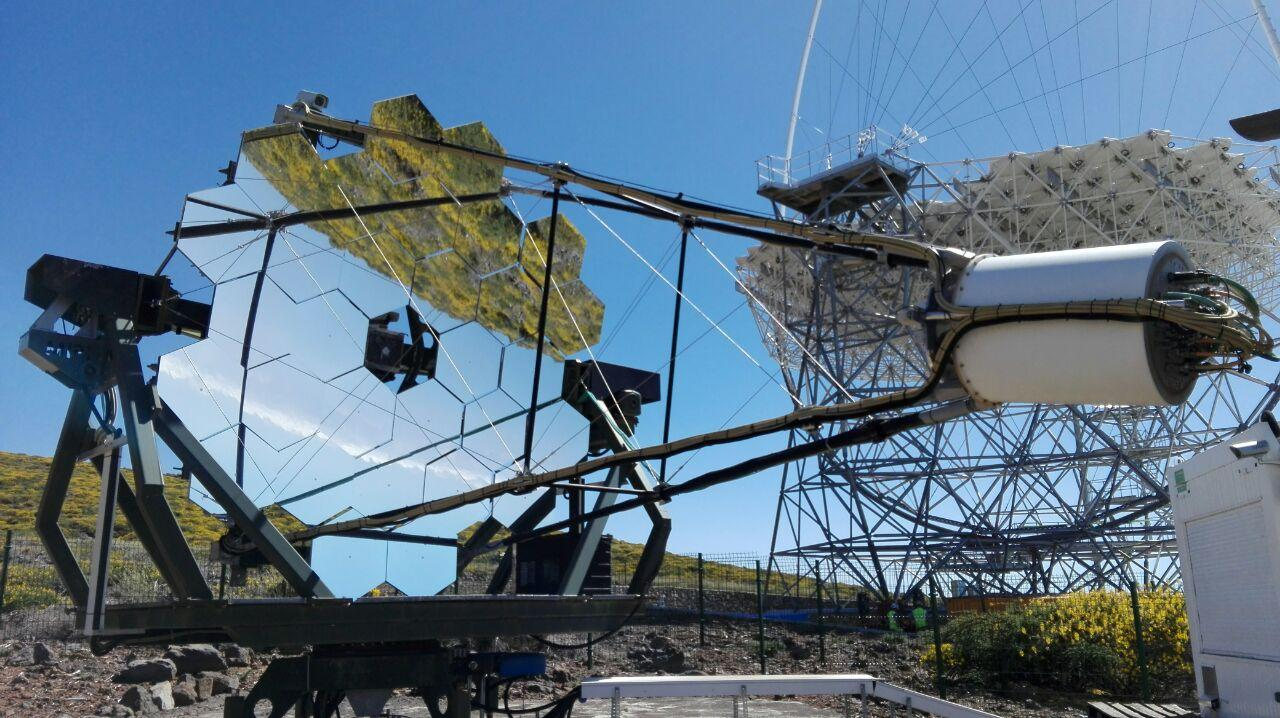
\includegraphics[width=\textwidth]{Plots/fact.jpg}
  \label{fig:fact}
  \caption{The First G-APD Cherenkov Telescope on the Observatory on the Roque des los Muchachos on the island of La Palma. Image courtesy of Kevin Schmidt.}
\end{figure}
%
The First G-APD Cherenkov Telescope \cite{FACT-Design} (FACT) is an IACT
protoype located $\SI{2200}{\metre}$ above sea-level on the Canary island of La
Palma. It measures air-shower-photons from cosmic gamma-rays with energies from
several hundred GeV up to about $\SI{10}{\tera\electronvolt}$. FACT uses a
segmented imaging-reflector with a $\SI{9.5}{\meter\squared}$ aperture and
$\SI{4.889}{\meter}$ focal-length. Apart from monitoring bright sources of
cosmic gamma-rays, like Markarian 421 and Markarian 501, FACT is used for
demonstrating and testing the usage of new technologies in the field of IACTs.

As the name suggests, FACT uses a novel kind of detector made of so called
Geiger-mode avalanche photodiodes (G-APD). The 1440 pixels of Silicon-Photo-Multipliers (SiPM), FACT uses to sense photons comprise these photomultipliers.
Each pixel yields about $\SI{0.1}{\degree}$ field-of-view, giving FACT
a total field-of-view of $\SI{4.5}{\degree}$. Using SiPMs instead of
Photo-Multiplier-Tubes (PMTs) differentiates FACT from other IACTs and gives it
special possibilities. SiPMs are very robust, compared to PMTs and can operate
in brighter light. This makes continuos observations even during bright moon
possible. The SiPMs furthermore have a photon detection efficiency comparable to those in PMTs and therefore the potential to replace PMTs in IACTs. FACT is sampling recorded
events with a frequency of $\SI{2}{\giga\hertz}$, giving it a very good time
resolution. The usual trigger rate during data taking lies between \num{50} - \SI{60}{\hertz} \cite{FACT-Design}. With these assets, FACT is well suited for long-term monitoring of
sources, finding flares and informing the astronomic community of such.
